\documentclass[11pt a4paper]{article}
\usepackage[margin=2cm]{geometry}
\usepackage{amsmath, amssymb}
\usepackage{graphicx}
\usepackage{float}
\usepackage{aligned-overset}
\usepackage{subcaption}

% partielle ableitungen
\newcommand{\delr}{\partial_r}
\newcommand{\deltheta}{\partial_\theta}
\newcommand{\delphi}{\partial_\varphi}

% elektrische feldkonstante
\newcommand{\epsz}{\epsilon_0}
% 1 / 4pi eps
\newcommand{\kco}{\frac{1}{4\pi\epsilon_0}}

% fancy header
\usepackage{fancyhdr}
\fancyhf{}
% vspaces in den headern fuer Distanzen notwendig
% linke Seite: Namen der Abgabegruppe
\lhead{\textbf{Matthias Maile\\Roman Surma}\vspace{1.5cm}}
% rechte Seite: Modul, Gruppe, Semester
\rhead{\textbf{Physik II - Gruppe 2\\Sommersemester 2020}\vspace{1.5cm}}
% Center: nr. des blattes
\chead{\vspace{2.5cm}\huge{\textbf{17. Übungsblatt}}}
% benoetigt damit der eigentliche Text nicht in der Überschrift steckt
\setlength{\headheight}{4cm}

% zum zeichnen tikz
\usepackage{tikz}

% fuer fabigen text
\usepackage{xcolor}

\begin{document}
\thispagestyle{fancy}
\section*{Aufgabe 1}
a) 
Für die Feldenergie betrachten wir das $E$-Feld im Kondensator. Da wo sich
das Dielektrikum befindet, ist das Feld $\frac{U}{d e_r}$, im restlichen 
Bereich $\frac{U}{d}$.
\[
	E(\vec r, x) = \begin{cases}
		\frac{U}{e_r d} &\text{für } \vec r \in A(x) \\
		\frac{U}{d} 	&\text{sonst} \end{cases}
\]
Dabei ist $A(x)$ die freie Fläche, welche natürlich von der Auslenkung $x$ 
abhängt.\\
Diesen Zusammenhang löst man am einfachsten grafisch:
\begin{center}
\begin{tikzpicture}
	% erste flaeche
	\filldraw[fill=green!20] 
		(-2,-2) -- (-2,2) -- (-1.5,2) -- (-1.5,-2);
	% zweite flaeche
	\filldraw[fill=blue!20]
		(-1.5,-2) -- (-1.5, 0) -- (0.5,-2);
	\filldraw[fill=blue!20]
		(-1.5,2) -- (-1.5, 0) -- (0.5,2);
	% dritte flaeche
	\filldraw[fill=red!20]
		(0.5, -2) -- (2,-0.5) -- (2,-2);
	\filldraw[fill=red!20]
		(0.5, 2) -- (2, 0.5) -- (2, 2);
	% kondensator und dielektrikum als zweites damit die raender orange
	% und schwarz sind
	% der kondensator
	\draw[gray, thick] (-2,2) -- (2,2);
	\draw[gray, thick] (-2,2) -- (-2,-2);
	\draw[gray, thick] (-2,-2) -- (2,-2);
	\draw[gray, thick] (2,-2) -- (2,2);
	% das dielektrikum
	\draw[orange, thick] (0.5, 2) -- (2.5, 0);
	\draw[orange, thick] (2.5, 0) -- (0.5, -2);
	\draw[orange, thick] (0.5, -2) -- (-1.5, 0);
	\draw[orange, thick] (-1.5, 0) -- (0.5, 2);
	% annotations
	\draw (-2,0) node [left] {$\sqrt{2}a$};
	\draw (-1.75, -2) node [below] {$x$};
	\draw (-0.75, -2) node [below] {$\frac{a}{\sqrt2}$};
	\draw (1.25, -2) node [below] {$\frac{a}{\sqrt2} - x$};
	% seperation fuer anotations
	\draw [thick, dashed] (-2, -2) -- (-2, -2.1);
	\draw [thick, dashed] (-1.5, -2) -- (-1.5, -2.1);
	\draw [thick, dashed] (0.5, -2) -- (0.5, -2.1);
	\draw [thick, dashed] (2, -2) -- (2, -2.1);
\end{tikzpicture}
\end{center}
Dann folgt $A(x)$:
\begin{align*}
	A(x) = {\color{green!70} A_1(x)} 
	+ {\color{blue!50} A_2(x)}
	+ {\color{red!50} A_3(x)}
	&= x \cdot \sqrt2 a + \frac{a^2}2 +
		\left(\frac{a}{\sqrt2} - x\right)^2 \\
	% binomische formel
	&= x \cdot \sqrt2 a + \frac{a^2}2 +
		x^2 - 2 \cdot \frac{a}{\sqrt2} x + 
		\left(\frac{a}{\sqrt2} \right)^2 \\
	% kuerzen
	&= x^2 + a^2
\end{align*}
Die elektrische Feldenergie ist gegeben durch
\[
	W = \frac{\epsz}{2} \int_{\mathbb{R}^3} E^2(\vec r) d^3r 
\]
Die Energie des $E$-Feldes ermitteln wir durch Aufteilung des Bereiches
mit und ohne Dielektrikum.\\
Dadurch erhalten wir zwei Bereiche, für die das $E$-Feld homogen ist. Dank
der Homogenität müssen wir nicht mehr integrieren sondern können mit dem 
Volumen multiplizieren:
\begin{align*}
	W(x) &= \frac{\epsz}{2} \int_{\mathbb{R}^3} E^2(\vec r) d^3r \\
	% auteilung
	&= \frac{\epsz}{2} \left(
		\left(\frac{U}{\epsilon_r d}\right)^2 \cdot d \cdot A(x) +
		\frac{U^2}{d^2} \cdot d \cdot 2a^2 -
		\frac{U^2}{d^2} \cdot d \cdot A(x) \right) \\
	% vereinfachung
	&= \frac{\epsz U^2}{2d} 
	\left( \frac{A(x)}{\epsilon_r^2} + 2a^2 - A(x) \right)\\
	% kuerzen
	&= \frac{\epsz U^2}{2d} A(x) 
	\cdot \left(\frac{1}{\epsilon_r^2} -1\right) +
	\frac{\epsz U^2 a^2}{d}
\end{align*}

\newpage
\setlength{\headheight}{0cm}

Mit der Gleichung $F = -\vec\nabla W$ lässt sich die rückstellende Kraft
bestimmen:
\begin{align*}
	F = -\vec\nabla W &= -\partial_x \left(
	\frac{\epsz U^2}{2d} A(x) 
	\cdot \left(\frac{1}{\epsilon_r^2} -1\right) +
	\frac{\epsz U^2 a^2}{d} 
	\right) \cdot \hat x\\
	% ableiten
	&= -\frac{\epsz U^2}{d} \cdot \left(\frac{1}{\epsilon_r^2} -1
	\right) \cdot \vec x
\end{align*}

b) Mit dem Ergebnis für die rückstellende Kraft aus a) können wir die DGL 
aufstellen:
\begin{align*}
	F = m\ddot x
	&= -\frac{\epsz U^2}{d} \cdot \frac{1 - \epsilon_r^2}{\epsilon_r^2}
	\cdot x \\
	% fuer dgl umstellen
	\Leftrightarrow
	-\frac{\epsz U^2}{dm} \cdot \frac{1 - \epsilon_r^2}{\epsilon_r^2}
	\cdot x + \ddot x &= 0
\end{align*}
Diese besitzt eine uns bekannte Form mit der Lösung
\[
	x(t) = \alpha \cdot \exp\left(
	\sqrt{-\frac{\epsz U^2}{dm} \cdot \frac{1 - \epsilon_r^2}
	{\epsilon_r^2}}  \cdot i \cdot t \right)
\]
Die Oszillation hat die Periodendauer
\[
	T = \frac{2\pi}{\omega} = 2\pi \sqrt{\frac
	{\epsilon_r^2 \cdot d \cdot m}
	{\epsz \cdot U^2 \cdot (1 - \epsilon_r^2)}}
\]

\section*{Aufgabe 2}
\section*{Aufgabe 3}

a)
Mit der Formel für den elektrischen Widerstand können wir das Volumen der 
Konstruktion ermitteln:
\begin{align*}
	R &= \rho_r \cdot \frac{l}{A}, & V &= 6 \cdot l \cdot A \\
	\Rightarrow A &= \frac{\rho_r \cdot l}{R} \quad (1)
	& \overset{(1)}{\Rightarrow} V &= 6 \frac{\rho_r \cdot l^2}{R}
\end{align*}

Damit folgt das Gewicht:
\[
	m = \rho \cdot V = \frac{6 \cdot \rho \cdot \rho_r \cdot l^2}{R}
\]

Und der Preis:
\[
	\text{Preis} = k \cdot m = 120.30 \text{ Euro}
\]

\section*{Aufgabe 4}
a)
Die Gesamtkapzität der Schaltung lautet
\[
	\frac{1}{C_{ges}} = \frac{1}{C_1} + \frac{1}{C_1 + C_2}
\]

Dann können wir durch die Bedingung $C_{ges} = C_2$ bestimmen:
\begin{align*}
	\frac{1}{C_{ges}} = \frac{1}{C_2}
	&= \frac{1}{C_1} + \frac{1}{C_1 + C_2} \\
	% brueche zusammen fuhren
	&= \frac{C_1 + C_2 + C_1}{C_1 (C_1 + C_2)} \\
	% kehrwert bilden
	\Leftrightarrow
	C_2 &= \frac{C_1 (C_1 + C_2)}{2C_1 + C_2} \\
	% bruch aufloesen
	\Leftrightarrow
	C_2^2 + 2C_1C_2 &= C_1^2 + C_1C_2 \\
	% fuer pq formel umstellen
	\Leftrightarrow
	0 &= C_1^2 - C_1C_2 - C_2^2
\end{align*}

Mit der $pq$-Formel erhalten wir $C_1$:
\begin{align*}
	C_1 &= \frac{C_2}{2} \pm \sqrt{\frac{C_2^2}{4} + C_2^2} \\
	% wurzel aufloesen
	&= \frac{C_2}{2} \pm \sqrt{1.25} \cdot C_2 \\
	% negatives ergebnis streichen
	C_1 \geq 0 \Rightarrow
	&= \frac{C_2}{2} + \frac{5}{4} C_2 = \frac{7}{4} C_2
\end{align*}

\section*{Aufgabe 5}

a) Die Schaltung vereinfacht sich zu den zwei Zeitintervallen:
\begin{figure}[H]
	\centering
	\begin{subfigure}[b]{0.3\textwidth}
		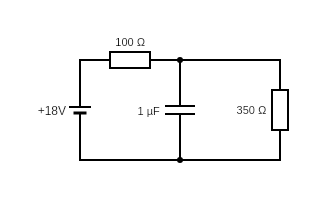
\includegraphics[width=5cm]{aufgabe5a_1.png}
		\caption{Für $t<0$}
	\end{subfigure}
	~
	\begin{subfigure}[b]{0.3\textwidth}
		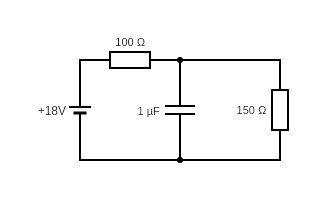
\includegraphics[width=5cm]{aufgabe5a_2.png}
		\caption{Für $t\geq0$}
	\end{subfigure}
\end{figure}
Wenn wir die Schaltungen als Spannungsteiler betrachten erhalten wir $U_C$ 
für $t < 0$ und $t \rightarrow \infty$:
\begin{align*}
	U_C (t < 0) &= \frac{350 \Omega}{100 \Omega + 350 \Omega} \ U_q
	&
	U_C (t\rightarrow\infty) &= \frac{150\Omega}{100\Omega +
	150 \Omega} \ U_q\\
	% brueche kuerzen
	&= \frac{350}{450} \ U_q & &= \frac{150}{350} \ U_q \\
	% spannungen ermitteln
	&= 14V & &=10.8V
\end{align*}
D.h. wenn bei $t=0$ der Schalter geschlossen wird, ist auf den 
Kondensatorplatten ein Potential von $14V$, während von der Spannungsquelle
nur noch $10.8V$ wirken.\\
Die `wirkende` Potentialdifferenz des Kondensators für $t=0$ lautet somit
\[ U_\text{Cap} (0) = 14V - 10.8V = 3.2V \]
Da sich der Kondensator am Widerstand $R_3 = 150\Omega$ entlädt lautet die
die Potentialdifferenz die aus dem Kondensator folgt:
\[
	U_\text{Cap} (t) = U_\text{Cap} (0) \cdot e^{\frac{-t}{\tau}}
	= U_\text{Cap} (0) \cdot e^{\frac{-t}{R_3 C}}
	= 3.2 V \cdot \exp\left(\frac{-t}{150\Omega \mu F}\right)
\]
Zusammen mit der Spannungsquelle existiert die Potentialdifferenz $U_C(t)$:
\[
	U_C = 10.8V + U_\text{Cap} (t) = 
	10.8V + 3.2 V \cdot  \exp\left( -\frac{2t}{3s} \cdot 10^4\right)
\]






\end{document}
